\chapter{Issues surrounding Markdown}
\label{chap:issues}

\vspace{1cm}

Markdown achieved its objectives of readability and simplicity, which were the main arguments for its fast rise in popularity.
What started as a simple Perl script that converts Markdown to HTML via regex replacements became a phenomenon, and was adopted in many
famous online services and pieces of software. However, there is no real ``specification'' for Markdown beyond the original blog post
introducing the language and a few other pages on Gruber's website.\footcite{gruber2004markdown}
With time, one of Markdown's strengths, it's simplicity, also became one of its flaws for a few reasons:

\begin{itemize}
    \item While integrating Markdown, many developers realised that unfortunately the official Perl script is filled with unintentional errors
    and breaking states, which generate invalid HTML;
    \item Users feel that some necessary features are missing;
    \item Other output formats than HTML were often requested, chiefly PDF.
\end{itemize}

These issues led to various implementations and syntaxes appearing all over the web-space (see chapter \ref{chap:proliferation}),
most of them incompatible with each other.

\section{Errors}

\section{Missing features}

\begin{itemize}
    \item Limited formatting options
    \item Lack of tables and footnotes
    \item Lack of accessibility
    \item No support for Macros or Variables
    \item Lack of metadata
    \item GFM: task lists, tables, and syntax highlighting for code blocks
\end{itemize}

\section{Output formats}

% TODO:
% Discuss Pandoc, Github flavored markdown, etc

\newpage

\section{One syntax, many implementations}

The will of the people to "fix" Markdown led to hundreds of implementations of it existing in the wild. All of these take opinionated stances
in how to fix the language, and of course most of them disagree on how. The lack of a proper Markdown standard specification led to dozens of
it now existing.\newline

Indeed, even extremely simple examples of Markdown documents lead to many different HTML outputs depending on the type of implementation used
to interpret the markdown snippet. In order to visualise the absurdity of it all, \citeauthor{babelmark} created a tool called "Babelmark"
(named after the Tower of Babel and the ``confusion of languages'') which allows to take a Markdown document and list all known HTML outputs
one would have with all the tools available online. On figure \ref{fig:babelmark}, we see a simple example of a markdown text: two headings of
level 1 and 2, with no other text. Even this short document leads to six different HTML outputs (three of which are shown in the figure).

\begin{figure}[H]
\centering
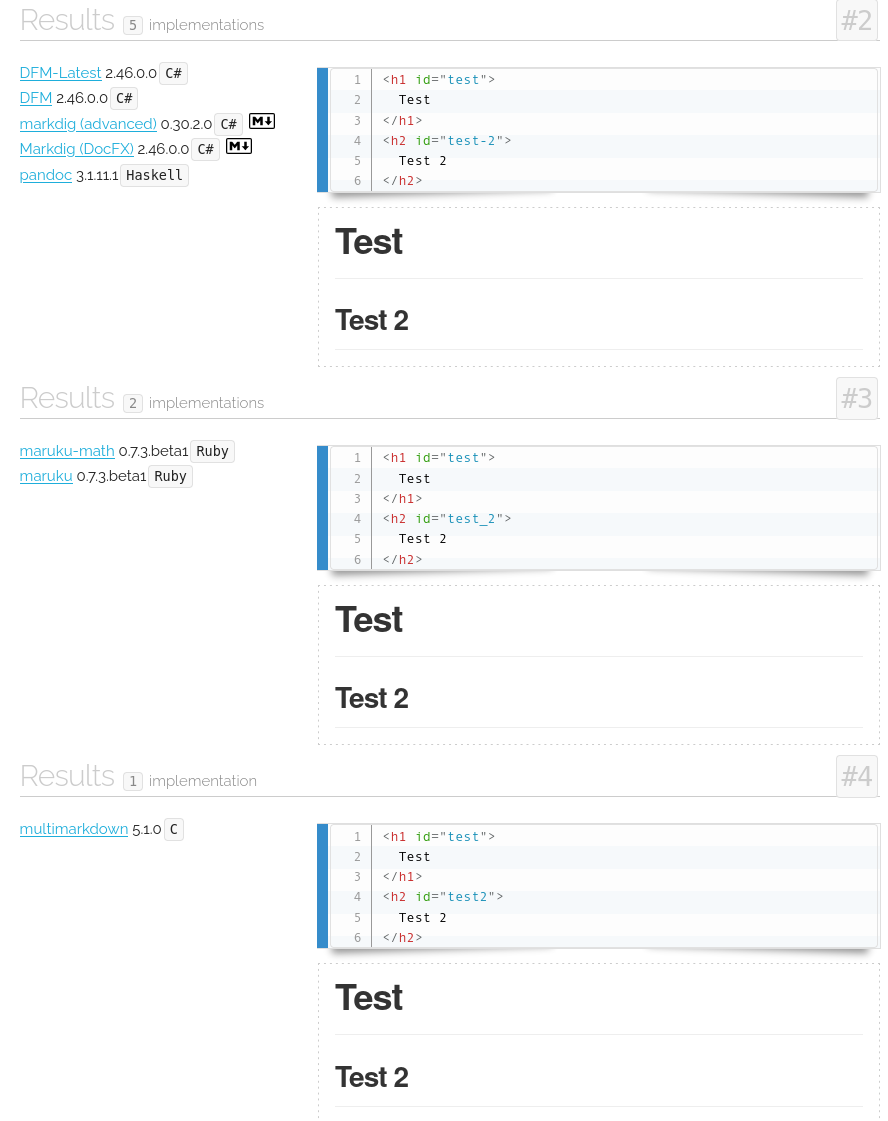
\includegraphics[scale=0.25]{babelmark}
\caption{Babelmark listing some of many possible outputs from markdown implementations}
\label{fig:babelmark}
\end{figure}

This lack of common ground led a group of people to push for a standard specification of Markdown to be created.

\section{Standardization efforts}

\cite{leonard2016text}

\cite{commonmark}